% Reporte: Medición del Radio de la Tierra — Método de Eratóstenes
% Curso: Introducción a la Astronomía Práctica
% Autores: Jean Lucca Buritica Cuervo, Daniel Soto Villada, Camilo Higuita

\documentclass[stu,12pt,floatsintext]{apa7}

\usepackage[spanish]{babel}
\usepackage{csquotes}
\usepackage[style=apa,sortcites=true,sorting=nyt,backend=biber]{biblatex}
\DeclareLanguageMapping{spanish}{spanish-apa}
\addbibresource{bibliography.bib}

\usepackage[T1]{fontenc}
\usepackage{mathptmx}
\usepackage{amsmath}
\usepackage{booktabs}
\usepackage{graphicx}

\title{Midiendo el planeta: reproducción moderna del método de Eratóstenes}
\shorttitle{Método de Eratóstenes}
\author{Jean Lucca Buritica Cuervo, Daniel Soto Villada y Camilo Higuita}
\duedate{5 de abril de 2026}
\affiliation{Universidad de Antioquia}
\course{Introducción a la Astronomía Práctica}
\professor{Por definir}

\abstract{Se reproduce el experimento de Eratóstenes para estimar el radio de la Tierra
midiendo la longitud de la sombra de un gnomon al mediodía solar en Medellín, Colombia
($\varphi = 6{,}2666°\,\text{N}$, $\lambda = -75{,}5694°\,\text{O}$).
Las mediciones se realizaron el 19 y el 20 de marzo de 2026, este último día correspondiente
al equinoccio de primavera. A partir de un ajuste parabólico sobre los datos de sombra se
determinó la longitud mínima de cada sesión y, mediante trigonometría y propagación de
incertidumbres, se calculó el ángulo cenital del Sol al mediodía. Usando el ecuador como
punto de referencia celeste se obtuvo un radio terrestre de $(6310{,}5 \pm 99{,}1)$ km
para el conjunto del equinoccio (error relativo $0{,}95\,\%$ respecto al valor de referencia
de $6371$ km) y de $(6132{,}1 \pm 176{,}0)$ km para el conjunto del día anterior (error
relativo $3{,}75\,\%$). Los resultados son consistentes con el valor aceptado dentro de sus
incertidumbres y demuestran la viabilidad del método en latitudes bajas.}

\begin{document}
\maketitle

% ─────────────────────────────────────────────────────────────────────────────
\section{Introducción}

En el siglo \textsc{iii} a.C., Eratóstenes de Cirene (c.\ 276–195 a.C.) estimó la
circunferencia de la Tierra comparando las sombras del gnomon en Alejandría y Siena al
mediodía del solsticio de verano \parencite{britannica_eratosthenes_2026}. La clave del
método es que, si la Tierra es esférica y los rayos del Sol llegan paralelos, la
diferencia del ángulo cenital entre dos puntos del mismo meridiano es igual al ángulo que
subtienden en el centro del planeta (véase la Figura~\ref{fig:esquema}).

\begin{figure}[h]
    \centering
    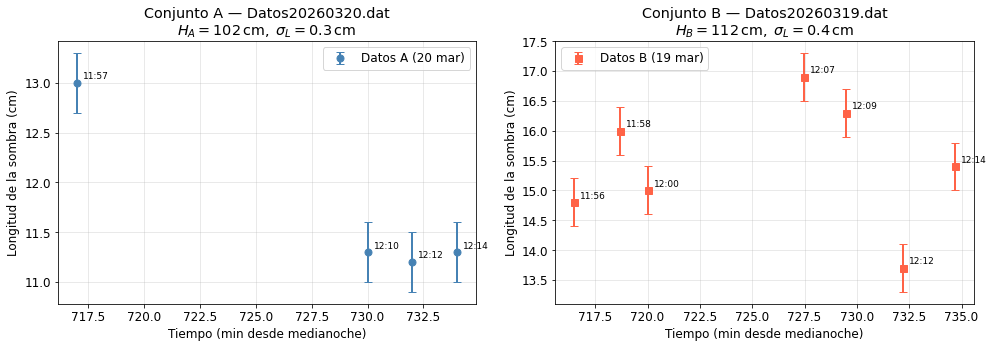
\includegraphics[width=0.65\linewidth]{../Analisis/figuras/sombras_datos_brutos.png}
    \caption{Longitud de la sombra del gnomon en función del tiempo para los dos conjuntos de datos.
             El mínimo de cada curva corresponde al mediodía solar.}
    \label{fig:esquema}
\end{figure}

Este trabajo reproduce el experimento con medios modernos, tomando como punto de referencia
el ecuador terrestre y aprovechando que el equinoccio de primavera de 2026 ocurrió el 20 de
marzo: en esa fecha la declinación solar es $\delta \approx 0°$, de modo que el Sol alcanza
su cénit exactamente sobre el ecuador al mediodía solar. Un día antes, el 19 de marzo,
$\delta \approx -0{,}48°$, lo que requiere una pequeña corrección geométrica pero no invalida
el método \parencite{noaa_solcalc}.

\subsection*{Objetivo}

Estimar el radio de la Tierra a partir de mediciones del gnomon realizadas en Medellín
durante los días 19 y 20 de marzo de 2026, y evaluar la concordancia del resultado
con el valor de referencia $R_{\oplus,\,\text{ref}} = 6371$ km.

% ─────────────────────────────────────────────────────────────────────────────
\section{Marco Teórico}

\subsection{Ángulo cenital al mediodía solar}

Un gnomon vertical de altura $H$ proyecta una sombra de longitud $L$ que es mínima en el
instante del mediodía solar (máxima elevación del Sol). El ángulo cenital $\theta_z$ en ese
instante se obtiene mediante:

\begin{equation}
    \theta_z = \arctan\!\left(\frac{L_{\min}}{H}\right).
    \label{eq:zenith}
\end{equation}

\subsection{Propagación de incertidumbres}

Aplicando la regla estándar de propagación de incertidumbres \parencite{jcgm2008gum} a la
ecuación~\eqref{eq:zenith}:

\begin{equation}
    \sigma_{\theta_z} = \frac{\sqrt{H^2\,\sigma_{L_{\min}}^2 + L_{\min}^2\,\sigma_H^2}}
                             {H^2 + L_{\min}^2}.
    \label{eq:prop_error}
\end{equation}

\subsection{Corrección por declinación solar}

El 19 de marzo de 2026 la declinación solar es $\delta \approx -0{,}48°$. El punto
sub-solar no está en el ecuador sino a latitud $\delta$, por lo que la distancia meridional
de referencia es:

\begin{equation}
    d_B = (\varphi - \delta)\,M_1,
    \label{eq:dist_corr}
\end{equation}

donde $M_1 = 110{,}574$ km/grado es la longitud de arco por grado de latitud en el
elipsoide WGS-84 \parencite{nga_wgs84}. Para el equinoccio ($\delta = 0$), simplemente
$d_A = \varphi\,M_1$.

\subsection{Radio y circunferencia de la Tierra}

Con la distancia meridional $d$ y el ángulo cenital en radianes, la regla de tres
geométrica da:

\begin{equation}
    R_\oplus = \frac{d}{\theta_z},
    \qquad
    C_\oplus = 2\pi R_\oplus,
    \label{eq:radio}
\end{equation}

con incertidumbres $\sigma_R = \dfrac{d}{\theta_z^2}\,\sigma_{\theta_z}$ y
$\sigma_C = 2\pi\,\sigma_R$.

% ─────────────────────────────────────────────────────────────────────────────
\section{Metodología}

\subsection{Participantes}

Las mediciones fueron realizadas por Jean Lucca Buritica Cuervo, Daniel Soto Villada y
Camilo Higuita como parte de la asignatura Introducción a la Astronomía Práctica.

\subsection{Materiales}

\begin{itemize}
    \item Gnomon (vara rígida) de $(112{,}0 \pm 0{,}1)$ cm (sesión del 19 de marzo).
    \item Gnomon de $(102{,}0 \pm 0{,}1)$ cm con soporte estable al suelo (sesión del 20 de marzo).
    \item Cinta métrica con resolución de 1 mm.
    \item Nivel de burbuja y plomada para verificar la verticalidad.
    \item Reloj sincronizado con UTC−5.
\end{itemize}

\subsection{Procedimiento}

Se eligió un área plana con exposición directa al Sol en Medellín (coordenadas
GPS: $\varphi = 6{,}2666°\,\text{N}$, $\lambda = -75{,}5694°\,\text{O}$).
El gnomon se fijó verticalmente y se tomaron varias mediciones de la longitud de la sombra
proyectada entre las 11:55 y las 12:15 (hora local UTC−5), abarcando un intervalo
de aproximadamente ±15 minutos alrededor del mediodía solar teórico (12:02, calculado a
partir de la longitud geográfica).

Los intervalos entre medidas fueron irregulares porque la cobertura nubosa intermitente
impedía obtener sombra nítida en todo momento. Cada observación consistió en medir la
longitud de la sombra desde la base del gnomon hasta su extremo, registrando también la
hora exacta.

\subsubsection*{Errores instrumentales}

Para el Conjunto~A (20 de marzo) se asignó un error de $\sigma_L = 0{,}3$ cm, asociado
principalmente al grosor del gnomon que produce sombras con penumbra. Para el
Conjunto~B (19 de marzo) se usó $\sigma_L = 0{,}4$ cm, valor mayor por las dificultades
de mantener la verticalidad del gnomon sin soporte rígido.

% ─────────────────────────────────────────────────────────────────────────────
\section{Análisis de Datos}

\subsection{Determinación del mediodía solar}

Cerca del mediodía solar la longitud de la sombra sigue una parábola:

\begin{equation}
    L(t) = a\,(t - t_0)^2 + L_{\min},
    \label{eq:parabola}
\end{equation}

donde $t_0$ es el instante del mediodía solar (en minutos desde medianoche) y $L_{\min}$ es
la longitud mínima de la sombra. Se ajustó esta función mediante mínimos cuadrados
ponderados (con peso $1/\sigma_L^2$) usando la rutina \texttt{curve\_fit} de SciPy
\parencite{virtanen2020scipy}.

Para el Conjunto~B el ajuste con todos los siete puntos produjo un coeficiente $a < 0$
(parábola invertida, físicamente imposible), situación atribuible a la dispersión
adicional por la inestabilidad del gnomon. Se restringió entonces el ajuste a los tres
puntos más próximos al mínimo aparente, que son los menos afectados por errores de
posicionamiento, obteniendo un ajuste exacto (tres parámetros, tres puntos).

Los ajustes parabólicos se muestran en las figuras~\ref{fig:ajusteA} y~\ref{fig:ajusteB}.

\begin{figure}[h]
    \centering
    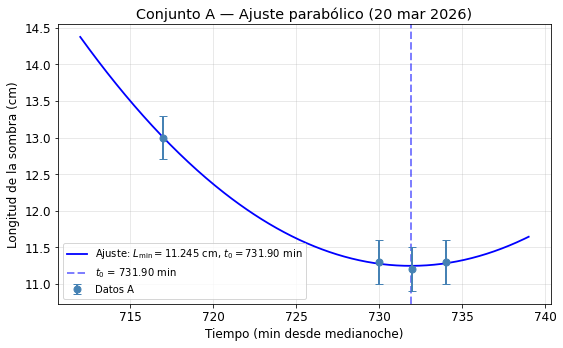
\includegraphics[width=0.72\linewidth]{../Analisis/figuras/ajuste_parabolico_A_20260320.png}
    \caption{Ajuste parabólico para el Conjunto~A (20 de marzo de 2026, equinoccio).
             Las barras de error representan $\sigma_L = 0{,}3$ cm.
             El mínimo del ajuste corresponde al mediodía solar.}
    \label{fig:ajusteA}
\end{figure}

\begin{figure}[h]
    \centering
    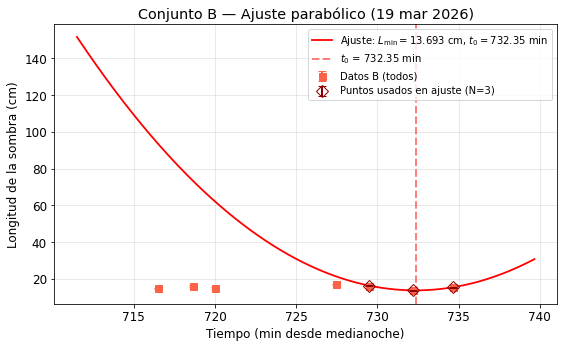
\includegraphics[width=0.72\linewidth]{../Analisis/figuras/ajuste_parabolico_B_20260319.png}
    \caption{Ajuste parabólico para el Conjunto~B (19 de marzo de 2026).
             Se utilizaron los tres puntos más cercanos al mínimo.
             Las barras de error representan $\sigma_L = 0{,}4$ cm.}
    \label{fig:ajusteB}
\end{figure}

\subsection{Resultados del ajuste}

Los parámetros obtenidos son:

\begin{itemize}
    \item \textbf{Conjunto A:} $L_{\min} = (11{,}245 \pm 0{,}178)$ cm,
          $t_0 = 731{,}9$ min (12:11:54), $\chi^2_\text{red} = 0{,}035$.
    \item \textbf{Conjunto B:} $L_{\min} = (13{,}693 \pm 0{,}397)$ cm,
          $t_0 = 732{,}3$ min (12:12:21) (ajuste exacto con tres puntos).
\end{itemize}

El $\chi^2_\text{red} \approx 0{,}035$ del Conjunto A, notablemente menor que 1, indica
que los errores declarados sobreestiman la dispersión real de esos cuatro puntos, o bien que
los datos muestran una consistencia excepcional. En cualquier caso, la incertidumbre
$\sigma_{L_{\min}}$ propagada desde la covarianza del ajuste es la que se usa en los pasos
siguientes \parencite{baird1991experimentacion}.

\subsection{Ángulo cenital y radio de la Tierra}

Usando las ecuaciones~\eqref{eq:zenith}–\eqref{eq:radio} y la longitud de arco
$M_1 = 110{,}574$ km/grado \parencite{nga_wgs84}, se obtienen los resultados
resumidos en la Tabla~\ref{tab:resultados}.

\begin{table}[h]
    \caption{Resumen de los parámetros del experimento y los resultados finales.}
    \label{tab:resultados}
    \centering
    \small
    \begin{tabular}{lcc}
        \toprule
        \textbf{Parámetro} & \textbf{Conj.~A (20 mar)} & \textbf{Conj.~B (19 mar)} \\
        \midrule
        Gnomon $H$ (cm)           & $102{,}0 \pm 0{,}1$ & $112{,}0 \pm 0{,}1$ \\
        $\sigma_L$ (cm)           & $0{,}3$             & $0{,}4$              \\
        Declinación $\delta$ (°)  & $0{,}00$            & $-0{,}480$           \\
        $\theta_z$ esperado (°)   & $6{,}2666$          & $6{,}7466$           \\
        $L_{\min}$ (cm)           & $11{,}245 \pm 0{,}178$ & $13{,}693 \pm 0{,}397$ \\
        $\theta_z$ medido (°)     & $6{,}291 \pm 0{,}099$  & $6{,}970 \pm 0{,}200$ \\
        $d$ (km)                  & $692{,}92$          & $745{,}99$           \\
        $R_\oplus$ (km)           & $6310{,}5 \pm 99{,}1$ & $6132{,}1 \pm 176{,}0$ \\
        $C_\oplus$ (km)           & $39650 \pm 623$     & $38529 \pm 1106$     \\
        Error relativo en $R$ (\%) & $0{,}95$           & $3{,}75$             \\
        \bottomrule
        \multicolumn{3}{l}{\footnotesize Referencia: $R_{\oplus,\text{ref}} = 6371{,}0$ km,
                            $C_{\oplus,\text{ref}} = 40030$ km.} \\
    \end{tabular}
\end{table}

% ─────────────────────────────────────────────────────────────────────────────
\section{Discusión}

\subsection{Concordancia con el valor de referencia}

El resultado del Conjunto~A, $R_\oplus = (6310{,}5 \pm 99{,}1)$ km, difiere del valor
de referencia $6371{,}0$ km en $\Delta R = 60{,}5$ km, equivalente a $0{,}6\,\sigma_R$.
Esta discrepancia es estadísticamente no significativa y puede considerarse un excelente
acuerdo para un experimento de bajo costo. El Conjunto~B arroja $R_\oplus = (6132{,}1 \pm 176{,}0)$ km,
con una desviación de $238{,}9$ km ($1{,}4\,\sigma_R$), valor aún compatible dentro de las
incertidumbres pero reflejo de las condiciones más adversas de medición.

\subsection{Fuentes de error}

\subsubsection*{Error sistemático por inclinación del gnomon (Conjunto B)}

La falta de soporte rígido en la sesión del 19 de marzo pudo introducir una inclinación
de hasta $1°$, lo que produciría un error sistemático en $L_{\min}$ del orden de
$H\sin(1°) \approx 2$ cm. Este efecto no está capturado por $\sigma_L$ y podría
explicar la mayor desviación respecto al valor teórico en ese conjunto.

\subsubsection*{Efecto del muestreo irregular}

Los intervalos entre medidas son irregulares por la cobertura nubosa. Esto no introduce
sesgo en $L_{\min}$ (el mínimo de una parábola no depende del espaciado de los puntos),
pero reduce la cobertura simétrica alrededor del mediodía solar y aumenta
$\sigma_{L_{\min}}$ \parencite{baird1991experimentacion}.

\subsubsection*{Corrección por declinación solar}

Omitir la corrección por declinación $\delta = -0{,}48°$ en el Conjunto~B equivaldría
a subestimar la distancia de referencia en
$|\delta| \times M_1 \approx 0{,}48° \times 110{,}574 \approx 53$ km, un $7{,}1\,\%$
del valor correcto. En latitudes bajas como la de Medellín esta corrección es necesaria.

\subsubsection*{Refracción atmosférica y extensión del disco solar}

A ángulos cenitales de $\approx 6°$ la refracción atmosférica es inferior a $0{,}01°$
y puede despreciarse. La extensión angular del Sol ($\approx 0{,}5°$) produce sombras con
penumbra, fuente principal del error $\sigma_L$ declarado \parencite{portilla2009elementos}.

\subsection{Comparación entre conjuntos}

El Conjunto~A ofrece mayor precisión ($\sigma_R/R \approx 1{,}6\,\%$) que el Conjunto~B
($\sigma_R/R \approx 2{,}9\,\%$). Esto se debe a tres factores combinados:
(a)~el soporte estable del gnomon, (b)~la proximidad del equinoccio que elimina la
corrección por declinación, y (c)~el menor error declarado $\sigma_L$.

% ─────────────────────────────────────────────────────────────────────────────
\section{Conclusiones}

Se logró medir el radio de la Tierra con una precisión del $0{,}95\,\%$ usando únicamente
un gnomon, una cinta métrica y mediciones tomadas durante aproximadamente 20 minutos al
mediodía solar. El resultado del Conjunto~A, $R_\oplus = (6310{,}5 \pm 99{,}1)$ km, es
compatible con el valor de referencia $6371{,}0$ km ($0{,}6\,\sigma_R$).

El experimento ilustra que el método de Eratóstenes, con más de dos milenios de antigüedad,
sigue siendo cuantitativamente válido con herramientas sencillas, siempre que se controlen
las fuentes de error sistemático más importantes: la verticalidad del gnomon y la
corrección por declinación solar cuando la medición no coincide con el equinoccio.

% ─────────────────────────────────────────────────────────────────────────────
\printbibliography

\end{document}
